\documentclass[10pt]{article}

\usepackage[margin=0.5in,bottom=.7in,top=.8in]{geometry}
\usepackage{graphicx}\graphicspath{{figures/}}
\usepackage[usenames,dvipsnames]{xcolor}
\usepackage[colorlinks=true,citecolor=Mahogany,linkcolor=Mahogany,urlcolor=Mahogany,filecolor=Mahogany]{hyperref}
\usepackage{breakurl}
\usepackage{url}
\usepackage[nocompress]{cite}
\usepackage{paralist}
\usepackage{authblk}
\usepackage{enumitem}
\usepackage{multirow}

\title{NLSR Developer's Guide}
\author[1]{Vince Lehman, Muktadir Chowdhury, Nicholas Gordon, Ashlesh Gawande}

\affil[1]{University of Memphis}

%\date{NFD Team}

\usepackage{fancyhdr}
\pagestyle{fancy}


\usepackage{eso-pic,xcolor}
\makeatletter
\AddToShipoutPicture*{%
\setlength{\@tempdimb}{20pt}%
\setlength{\@tempdimc}{\paperheight}%
\setlength{\unitlength}{1pt}%
%\put(\strip@pt\@tempdimb,\strip@pt\@tempdimc){%
%    \makebox(0,-60)[l]{\color{blue}%
%NDN, Technical Report NDN-0021. \url{http://named-data.net/techreports.html}}
%  }%
}
\makeatother


\begin{document}
\maketitle

\begin{abstract}
The Named Data Link-State Routing Protocol (NLSR) is a Named Data Networking (NDN) routing protocol that populates NDN Forwarding Daemon's (NFD) Routing Information Base (RIB).
The main design goal of NLSR is to provide a routing protocol to populate NFD's RIB and Forwarding Information Base (FIB).
NLSR calculates the routing table using link-state or hyperbolic routing and produces multiple faces for each reachable name prefix in a single authoritative domain.
NLSR will continue to evolve alongside the NDN protocol, NFD, and ndn-cxx.
This document is meant to explain the design of NLSR including major module and data structures descriptions and the interactions between those components.

\end{abstract}

\tableofcontents
\clearpage

\section{Introduction}
\label{sec:intro}

The Named-data Link State Routing protocol (NLSR) is an intra-domain routing protocol for Named Data Networking (NDN).
It is an application level protocol similar to many IP routing protocols, but NLSR uses NDN's Interest/Data packets to disseminate routing updates.
Although NLSR is designed in the context of a single domain, its design patterns may offer a useful reference for future development of inter-domain routing protocols.

NLSR supports name-based routing in NDN, computes routing ranks for all policy-compliant next-hops which provides a name-based multi-path routing table for NDN's forwarding strategy,
and ensures that routers can originate only their own routing updates using a hierarchical trust model.

\subsection{NLSR Modules and Data Structures}
\label{sec:modules}
NLSR contains multiple modules that each contribute to the total realization of the protocol.
Many of the modules interact with one another to trigger some behavior or to modify information in data structures.
NLSR uses the following modules:
\begin{itemize}
\item \textbf{Hello Protocol} (Section~\ref{sec:hello-protocol}) - determines the status of neighboring routers using periodic Hello Interests and notifies other modules when neighbors' statuses change.
\item \textbf{ChronoSync} - provides network-wide synchronization of NLSR LSDBs.~\cite{chronosync}
\item \textbf{Sync Logic Handler} (Section~\ref{sec:sync-logic}) - handles sync update notifications from NSync by retrieving updated LSAs.
\item \textbf{LSAs} (Section~\ref{sec:lsas}) - represent routing information published by the router.
\item \textbf{LSDB} (Section~\ref{sec:lsdb}) - stores the LSA information distributed by other routers in the network.
\item \textbf{Routing Table} (Section~\ref{sec:routing-table}) - calculates and maintains a list of next hops for each router in the network.
\item \textbf{Name Prefix Table} (Section~\ref{sec:npt}) - stores all advertised name prefixes and their next hops.
\item \textbf{FIB} (Section~\ref{sec:fib}) - maintains a shadow FIB which represents the intended state of NFD's FIB~\cite{NFD}.
\item \textbf{Prefix Update Processor} (Section~\ref{sec:prefix-update}) - listens for dynamic prefix announcements to advertise or withdraw name prefixes.
\item \textbf{NFD RIB Command Processor} (Section~\ref{sec:nfd-rib-commands}) - listens for readvertise-to-NLSR commands to advertise or withdraw name prefixes that were inserted into NFD.
\end{itemize}

\subsection{Protocol Overview}
\label{sec:protocol-overview}

NLSR is designed to accomplish three main tasks: (1) discover adjacent
neighbors; (2) disseminate and synchronize topology, name prefix, and
hyperbolic routing information; and (3) calculate a routing table and
populate NFD's FIB.  The entire protocol is described in detail in the
NLSR paper~\cite{NlsrTr}.

\subsubsection{Discovering Neighbors}

NLSR determines the adjacency status of neighboring routers using the Hello Protocol module (Section~\ref{sec:hello-protocol}).
When the Hello Protocol detects a status change for a neighbor, it will ask the LSDB module (Section~\ref{sec:lsdb}) to update the router's advertised adjacency information.

\subsubsection{Disseminating Routing Information}

When a router's LSAs (Section~\ref{sec:lsas}) changes, the information of this change should be distributed to every other router in the network.
The Sync Logic Handler module (Section~\ref{sec:sync-logic}) is used to notify the synchronization protocol of changes to the router's own LSAs as well as to learn of LSA changes from other routers in the network;
the Sync Logic Handler module interfaces with ChronoSync to perform the two tasks.

When the Sync Logic Handler module learns of a new LSA, it will inform the LSDB module.
The LSDB module will attempt to fetch the new LSA and will store it in the LSDB module's database if it can be retrieved.
If the newly fetched LSA informs the router of previously unknown routing information, the LSDB module will inform other modules depending on the type of routing information:
\begin{itemize}
  \item \textbf{Change in network topology} - the LSDB module will ask the Routing Table module (Section~\ref{sec:routing-table}) to recalculate paths in the network
\item \textbf{Change in name prefix advertisement} - the LSDB module will inform the Name Prefix Table module (Section~\ref{sec:npt}), which will in turn notify the FIB module (Section~\ref{sec:fib}) in order to add or remove the changed name prefixes.
\item \textbf{Change in hyperbolic coordinates} - the LSDB module will inform the Routing Table module (Section~\ref{sec:routing-table}), so the Routing Table module can calculate an up-to-date routing table.
\end{itemize}

\subsubsection{Calculating the Routing Table and Populating NFD's FIB}

When the routing table is calculated by the Routing Table module, the computed next hops are passed to the Name Prefix Table module.
The Name Prefix Table module will then further pass the next hops to the FIB module to update NLSR's expected state of NFD's FIB.
The FIB module will then perform the registrations or unregistrations with NFD's FIB.\\

A simplified diagram of NLSR's actions when receiving new routing information is shown in Figure~\ref{fig:system-interaction}.
The remainder of this documentation will describe the purpose of and interaction between each module in more detail.

\begin{figure}
\center
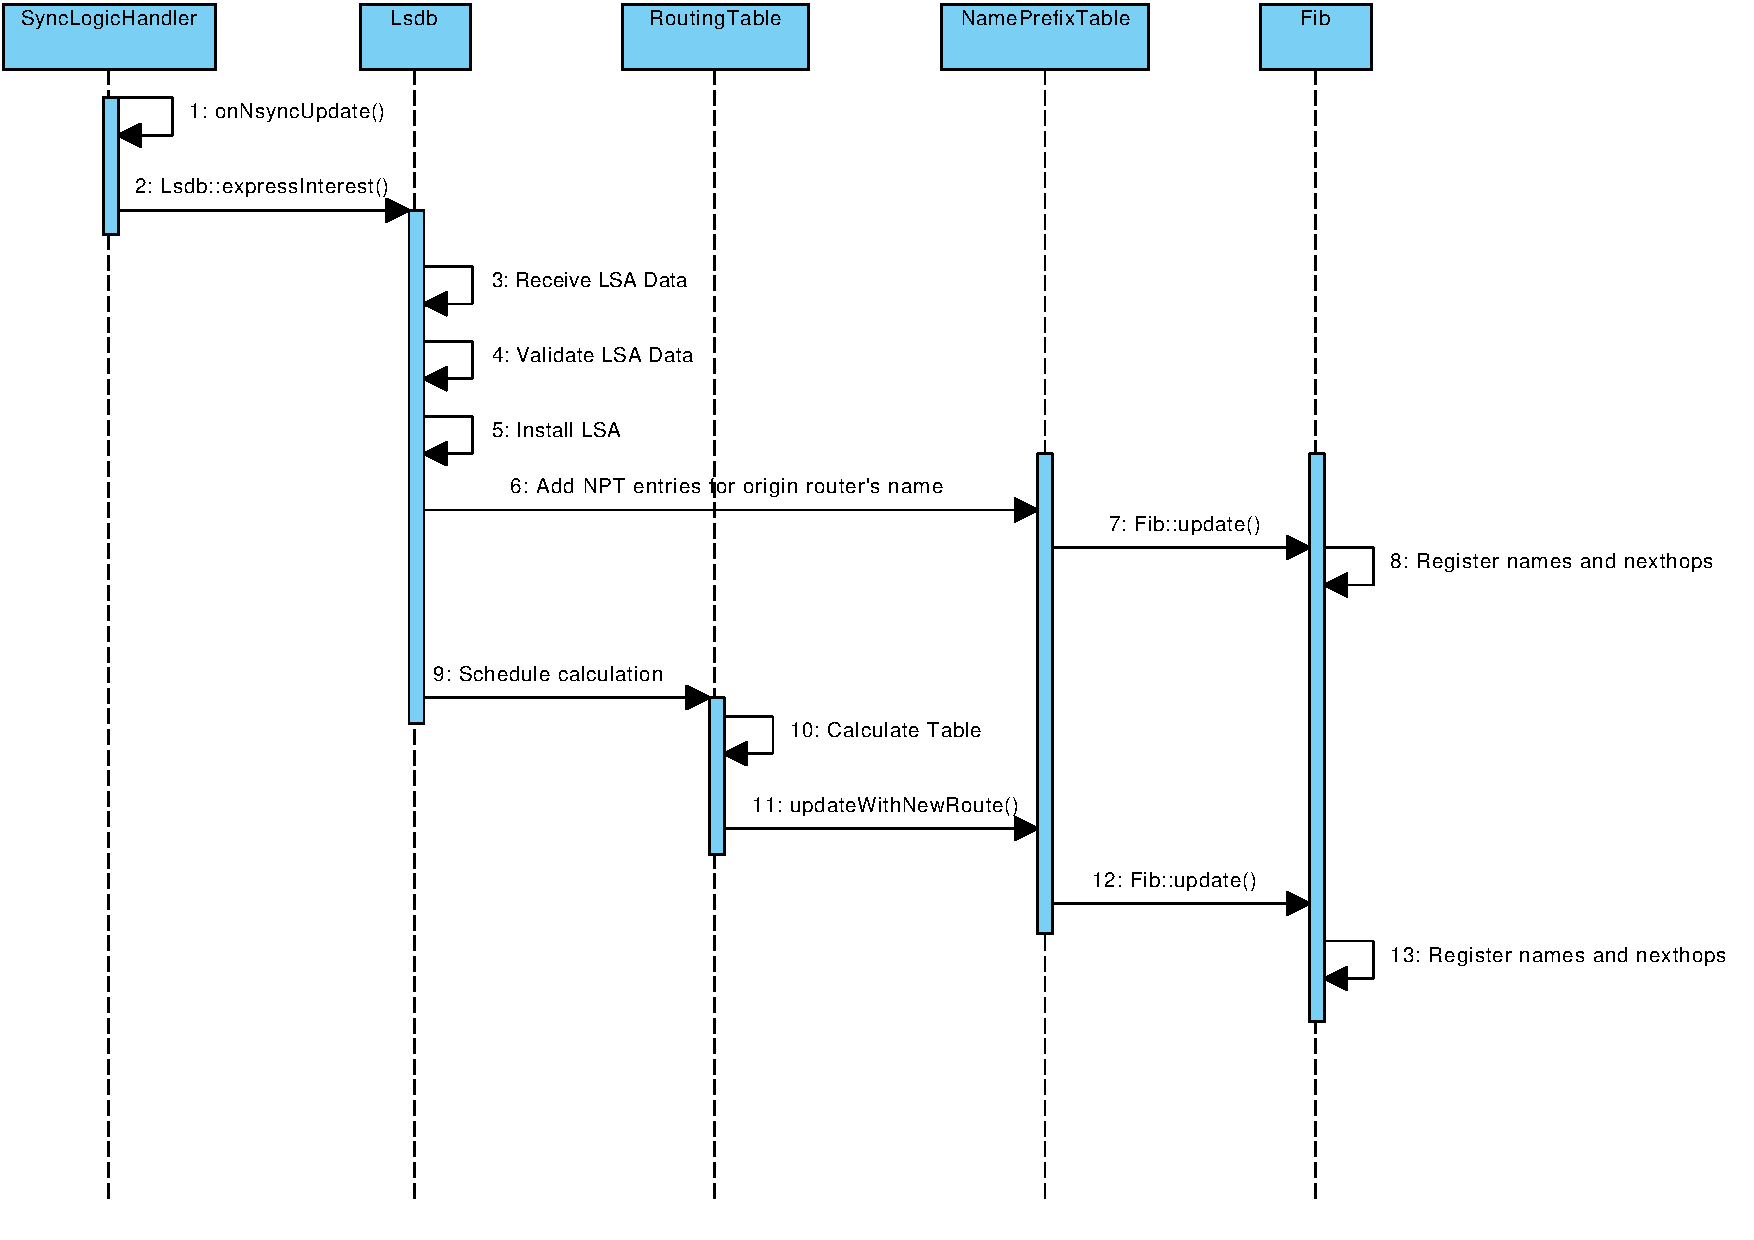
\includegraphics[width=\linewidth]{figures/system-interaction.pdf}
\caption{Simplified Diagram of the Actions of NLSR's Modules}
\label{fig:system-interaction}
\end{figure}

\subsection{Dispatcher}
\label{sec:dispatcher}

NLSR takes advantage of a variety of ndn-cxx convenience
mechanisms. Among these is the dispatcher. The dispatcher provides
facilities for receiving and decoding ControlCommands, which
simplifies the processing workflow. The dispatcher itself is
\href{http://named-data.net/doc/ndn-cxx/current/doxygen/de/d34/classndn_1_1mgmt_1_1Dispatcher.html}{well-documented},
so we will only give a brief overview here.

\begin{itemize}
\item Any prefixes that are registered, such as ``prefix/register'',
  \emph{must} be registered before top-level prefixes. All prefix
  registrations should go in \texttt{Nlsr::registerLocalhostPrefix}.
\item The dispatcher can be used to accept incoming ControlCommands
  and respond to requests for datasets. Currently NLSR uses the
  dispatcher only for accepting incoming ControlCommands.
\item Top-level prefixes cannot overlap. For example, you cannot
  register ``/localhost/nlsr'' and then ``/localhost/nlsr/fib''. The
  second registration must be done as a sub-prefix of the first,
  i.e. the first prefix, and then ``fib''.
\end{itemize}

\clearpage
\section{Hello Protocol}
\label{sec:hello-protocol}

The Hello Protocol module periodically sends Hello Interests to learn the activity status of the router's neighbors.
Hello Interests' names are constructed in the form: \texttt{/<neighbor's-router-prefix>/NLSR/INFO/<this-router's-prefix>}.
If a neighbor responds to a Hello Interest, the neighbor is considered to be up and \texttt{ACTIVE}.
A Hello Data's name is constructed using the following convention: \texttt{/<neighbor's-router-prefix>/NLSR/INFO/<this-router's-prefix>/<version>}.
If a neighbor fails to respond to a configurable number of Hello Interests (\texttt{hello-retries}), the neighbors is considered to be down and \texttt{INACTIVE}.
The Hello Protocol continues to send these periodic Hello Interests to each of its neighbors every \texttt{hello-interval} seconds.
If the Hello Protocol detects a change in a neighbors status
(i.e. a router that was previously \texttt{ACTIVE} is not responding to Hello Interests or a router that was previously \texttt{INACTIVE} responds to a Hello Interest),
it will notify the LSDB (Section~\ref{sec:lsdb}) to schedule a new Adjacency LSA build to include the updated neighbor information.

\subsection{Determining Neighbor's Status}
\label{sec:initial-status}

\begin{figure}
\center
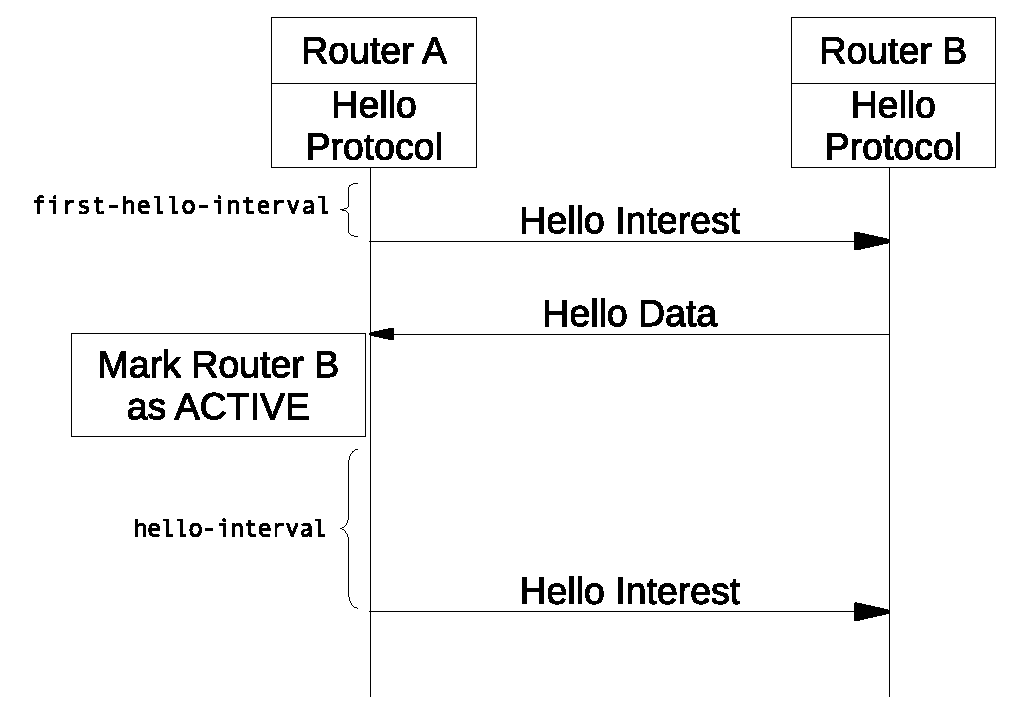
\includegraphics[width=0.5\textwidth]{figures/hello-protocol}
\caption{Router A determines the initial status of Router B}
\end{figure}

The Hello Protocol begins by scheduling Hello Interests to be sent to each neighbor of the router after \texttt{first-hello-interval} seconds.
When the scheduled event is triggered, the Hello Protocol iterates through the list of neighbors first checking if there is already a Face to the neighbor.
If there is a Face that has already been created, the Hello Protocol will construct and send a Hello Interest to the neighbor.
If a Face has not been created for the neighbor, the Hello Protocol will attempt to create a Face to the neighbor and register the neighbor's router prefix.
If the Face is created successfully, the Hello Protocol registers the Sync prefix, LSA prefix, and Key prefix using the Face ID returned by the Face creation command and sends out the Hello Interest.
If the Face cannot be created, the Hello Protocol considers the failure as a Hello Interest timeout.

If the Hello Protocol receives Data in response to its Hello Interest, it will first ask the Validator module to verify that the Data is valid. Data is valid if the Data is legitimately signed (in the ordinary cryptographic way) and if the key name and Data name are of a certain format.
If the Data is valid, the corresponding neighbor is set as \texttt{ACTIVE} and its timeout count is reset to zero.
If the neighbor was previously \texttt{INACTIVE}, an Adjacency LSA build is scheduled to include the newly \texttt{ACTIVE} neighbor.
If the Data is not valid, the packet is dropped.

If the Hello Interest sent to the neighbor times out, the corresponding neighbor's timed-out count is incremented.
If the neighbor's timed-out count is less than \texttt{hello-retries} in the configuration file, the Hello Protocol will send another Hello Interest after \texttt{hello-timeout} seconds.
If the neighbor's timed-out count equals the \texttt{hello-retries} value and the neighbor is currently marked as \texttt{ACTIVE}, the neighbor's status is set to \texttt{INACTIVE} and an Adjacency LSA build is scheduled.

\subsection{Responding to Hello Interests}
\label{sec:respond-to-hello}

If the Hello Protocol receives a Hello Interest from another router, it will first verify that the Hello Interest came from one of its configured neighbors.
If so, the Hello Protocol responds to the Interest with Hello Data.
To optimize the time to respond to link recoveries, the Hello Protocol will then immediately send a Hello Interest to the neighbor if the neighbor is currently marked as \texttt{INACTIVE}.

\subsection{Failure and Recovery Detection}
\label{sec:link-failure}

\begin{figure}
\center
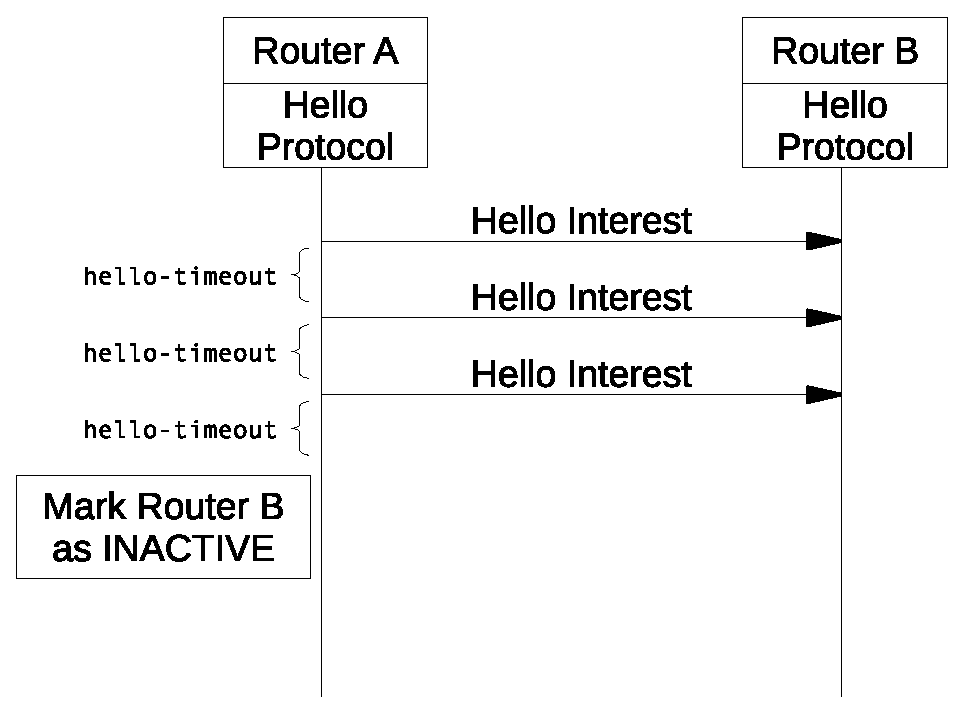
\includegraphics[width=0.5\textwidth]{figures/hello-protocol-timeout}
\caption{Router A determines that Router B has failed}
\end{figure}

The Hello Protocol will consider a neighbor as failed if the neighbor is currently \texttt{ACTIVE}, but Hello Interests sent to the neighbor have timed-out \texttt{hello-retries} number of times.
A failure can also be detected if a FaceEventNotification is received with the information that a Face to the neighbor has been destroyed.
The event is handled by the \texttt{Nlsr} class, but the triggered events simulate the actions of the Hello Protocol.
If the neighbor was currently \texttt{ACTIVE}, the neighbor will be set to \texttt{INACTIVE}, the neighbor's timed-out count will be set to \texttt{hello-retries}, and an Adjacency LSA build will be scheduled.

The Hello Protocol will consider a neighbor as recovered if the neighbor is currently \texttt{INACTIVE}, but the Hello Protocol has received valid Data in response to a Hello Interest sent to the neighbor.

\clearpage
\section{Sync Logic Handler}
\label{sec:sync-logic}

The Sync Logic Handler acts as the interface between the synchronization protocol and the NLSR application.
The Sync Logic Handler receives notifications from the synchronization protocol when another router updates an LSA, where an update can be modification of the contents of the LSA, or just incrementing the sequence number to refresh it. The  Sync Logic Handler then determines if the updated LSA should be retrieved. The Sync Logic Handler is also how NLSR notifies the sync protocol when its own LSAs are updated.

\subsection{On Sync Update}
When the sync protocol receives an update, the procedure roughly is this:
\begin{itemize}
\item For each name in the update:
\item Check that the sequence number in the LSA is newer than the one stored in the LSDB.
\item If so, tell the LSDB to fetch this new LSA. The LSDB will finish processing.
\end{itemize}

When the synchronization protocol receives a sync update, which may contain multiple distinct items, the names and sequence numbers of each item will be passed to \texttt{SyncLogicHandler::onNsyncUpdate()}.
%% This may not be necessary. It is currently true, though.
% The Sync Logic Handler will process each updated name individually first by verifying that the update is not for one of the router's own LSAs.
Since other syncs in the network blindly transmit what they think is new, we need to check that it's new \emph{to us}, and we use the LSA sequence number to do that. The higher sequence number of the locally-stored LSA with the same name as in the update and the sequence number in the update is taken to be the newer one, noting that an absent LSA has a sequence number of 0.
If the update is found to be newer, the Sync Logic Handler will call \texttt{Lsdb::expressInterest()}, which attempts to fetch the LSA represented by the update. Other LSDB methods will finish processing and installing the new LSA. (Section~\ref{sec:lsdb})

\subsection{Publish Routing Update}
\label{sssec:routing-update}
When any of a router's LSAs are updated or refreshed by the LSDB, the LSDB will use the \\ \texttt{SyncLogicHandler::publishRoutingUpdate()} method to notify the sync protocol that the sequence number for that LSA has changed.
The Sync Logic Handler will also write the updated sequence number to file, so that a restarting router can continue publishing routing updates with sequence numbers larger than the sequence numbers it had published before. This is only an optimization. If a router were to reset its sequence number to 1, other routers would initially reject these LSAs as not being new. However, the LSAs in their LSDBs would eventually expire, since they are not being refreshed anymore. Once those LSAs expire, the LSAs that the restarted router is publishing would then be considered new. However, this process could take quite a while, so we optimize by resuming numbering where we left off.

\clearpage
\section{Link-State Advertisements}
\label{sec:lsas}

Link-State Advertisements (LSAs) represent pieces of routing information distributed by routers.
NLSR uses three types of LSAs to distribute routing information:
Adjacency LSAs which include neighboring node and link information,
Coordinate LSAs which include a router's hyperbolic coordinates, and
Name LSAs which include advertised name prefixes reachable through the router.
All of the LSAs received by the router are maintained by the LSDB module (Section~\ref{sec:lsdb}).

\subsection{LSA Base Class}
\label{sec:lsa-base-class}

All three LSA implementations inherit from an LSA Base class, \texttt{Lsa}, which maintains information that is included in each LSA.
The \texttt{LSA} class contains the following member variables:
\begin{itemize}
\item \textbf{Origin Router} - the router that advertised the LSA.
\item \textbf{Sequence Number} - a number used to indicate the LSAs version as well as its ordering compared to other LSAs received from the same router.
\item \textbf{Expiration Time Point} - a time point indicating when the LSA is no longer valid.
\end{itemize}

\subsection{Adjacency LSAs}
\label{sec:adjacency-lsas}

Adjacency LSAs maintain an \texttt{AdjacencyList} which contains all the currently \texttt{ACTIVE} neighbors of the origin router.

\subsection{Coordinate LSAs}
\label{sec:coordinate-lsas}

Coordinate LSAs maintain the hyperbolic angle(s) and hyperbolic radius of the origin router.

\subsection{Name LSAs}
\label{sec:name-lsas}

Name LSAs maintain a \texttt{NamePrefixList} which contains advertised name prefixes that are reachable through the origin router.
\clearpage
\section{Link-State Database}
\label{sec:lsdb}

The Link-State Database (LSDB) holds LSA information distributed by other routers in the network.
The LSDB stores all three types of LSAs and will trigger necessary events when a new LSA is added, when an LSA is updated, and when an LSA expires.
The LSDB also handles LSA retrieval and validation, performs LSA builds, and triggers routing table calculations.

\subsection{Retrieving an LSA}

The LSDB provides \texttt{Lsdb::expressInterest()} as a public interface to retrieve an LSA from the network.
If LSA Data is returned, the LSDB will handle the Data validation and perform the necessary LSDB modifications.
If the LSA Interest times out, the LSDB will continue to re-attempt to fetch the LSA Data.
The LSDB will stop trying these fetch re-attempts once it has tried for as long as the maximum configurable LSA refresh time.

\subsection{Building LSAs}

The LSDB provides three interfaces to build and install a router's own various LSAs.
\begin{itemize}
\item \texttt{Lsdb::scheduleAdjLsaBuild()} schedules an Adjacency LSA calculation if one is not already scheduled and if hyperbolic routing is not turned on, i.e. if link-state routing or dry run is on.
\item \texttt{Lsdb::buildAndInstallOwnAdjLsa()} instantiates a new Adjacency LSA with the router's current adjacency list, incremented sequence number, and number of active neighbors. It also notifies the Sync Logic Handler to publish the routing update(Section~\ref{sssec:routing-update}) if link-state routing or dry-run is enabled to let other node in the network know the newly instlled Adjacency LSA.
\item \texttt{Lsdb::buildAndInstallOwnCoordinateLsa()} instantiates a new Coordinate LSA with the router's hyperbolic coordinates and an incremented sequence number. The newly constructed Coordinate LSA is then installed in the LSDB. It also notifies the Sync Logic Handler to publish the routing update(Section~\ref{sssec:routing-update}) if hyperbolic routing or dry run is turned on to let other nodes in the network know the newly installed Coordinate LSA.
\item \texttt{Lsdb::buildAndInstallOwnNameLsa()} instantiates a new Name LSA with the router's current name prefix list and an incremented sequence number. The newly constructed Name LSA is then installed in the LSDB.
\end{itemize}

\subsection{LSA Installation and Updates}

The LSDB provides three internal interfaces for each of the three types of LSAs to add or update LSAs in the LSDB.
The general logic for each type of LSA installation is similar (Figure~\ref{fig:generic-lsdb-flow}), but there are slight differences in the events that are triggered by an installation or update.

\begin{figure}
\center
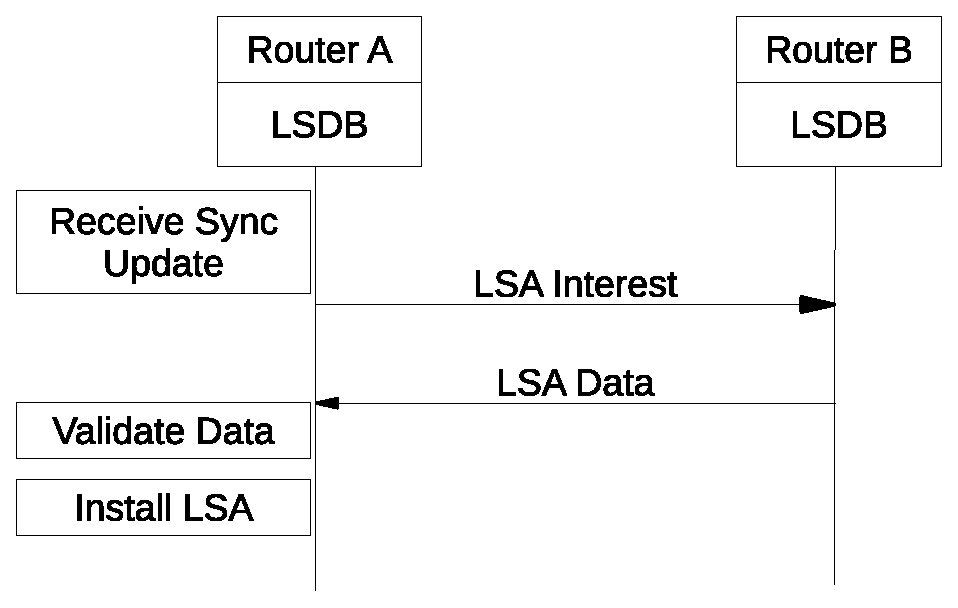
\includegraphics[width=0.5\linewidth]{figures/generic-lsdb-flow}
\label{fig:generic-lsdb-flow}
\caption{The general LSDB logic for each LSA type}
\end{figure}

\subsubsection{Lsdb::installAdjLsa()}

When an Adjacency LSA is passed to \texttt{Lsdb::installAdjLsa()}, the LSDB first attempts to find the LSA in its current database.

If the Adjacency LSA is not installed in the database, the LSA will first be added to the database.
If the installed LSA is advertised by a remote router, the remote router's name will be added to the NPT and the LSA will be scheduled to expire after the expiration time point included in the LSA.
Since a new Adjacency LSA introduces a new node and new links in the network, a routing table calculation is scheduled.

If the Adjacency LSA is already installed in the database, the existing LSA will only be updated if the newly received LSA has a higher sequence number.
If an Adjacency LSA with a higher sequence number is being installed, the existing LSA's sequence number and expiration time will be updated.
If the newly received LSA contains an adjacency list that is different from the existing LSA, the existing LSA's adjacencies are updated and a routing table calculation is scheduled to account for the network change.
Finally, if the updated LSA is advertised by a remote router, the LSA will be scheduled to expire after the expiration time point included in the LSA.

\subsubsection{Lsdb::installCoordinateLsa()}

When a Coordinate LSA is passed to \texttt{Lsdb::installCoordinateLsa()}, the LSDB first attempts to find the LSA in its current database.

If the Coordinate LSA is not installed in the database, the LSA will first be added to the database.
If the installed LSA is advertised by a remote router, the remote router's name will be added to the NPT, and the LSA will be scheduled to expire after the expiration time point included in the LSA.
If hyperbolic routing is enabled, a new Coordinate LSA means that the routing table should be re-calculated to include the new destination router.

If the Coordinate LSA is already installed in the database, the existing LSA will only be updated if the newly received LSA has a higher sequence number.
If a Coordinate LSA with a higher sequence number is being installed, the existing LSA's sequence number and expiration time will be updated.
If the newly received LSA contains hyperbolic coordinate different from the existing LSA, the existing LSA's coordinates are updated.
If hyperbolic routing is enabled, an LSA with new coordinates means the routing table should be re-calculated to account for the different coordinates.
Finally, If the updated LSA is advertised by a remote router, the LSA will be scheduled to expire after the expiration time point included in the LSA.

\subsubsection{Lsdb::installNameLsa()}

When a Name LSA is passed to \texttt{Lsdb::installNameLsa()}, the LSDB first attempts to find the LSA in its current database.

If the Name LSA is not installed in the database, the LSA will first be added to the database.
If the installed LSA is advertised by a remote router, the remote router's name and each advertised name in the LSA will be added to the NPT,  and the LSA will be scheduled to expire after the expiration time point included in the LSA.

If the Name LSA is already installed in the database, the existing LSA will only be updated if the newly received LSA has a higher sequence number.
If a Name LSA with a higher sequence number is being installed, the existing LSA's sequence number and expiration time will be updated.
A set difference is performed between the new LSA's advertised name prefix list and the existing LSA's advertised name prefix list to determine name prefixes that have been added.
If there are added name prefixes, the name prefixes are added to the NPT and to the existing LSA.
A set difference is then performed between the new LSA's advertised name prefix list and the existing LSA's advertised name prefix list to determine name prefixes that have been removed.
If there are removed name prefixes, the name prefixes are removed from the NPT and from the existing LSA.
Finally, If the updated LSA is advertised by a remote router, the LSA will be scheduled to expire after the expiration time point included in the LSA.

\subsection{LSA Expiration}

LSAs are scheduled to expire after a configurable amount of time in order to allow for LSDB cleanup when a router crashes.
After the expiration period, if the LSA belongs to the current router, the LSA is refreshed with an incremented sequence number (Section~\ref{sec:lsa-refresh}).
Otherwise, if the LSA belongs to a remote router, the LSA is removed from the LSDB.
Removing an LSA from the LSDB triggers different events depending on the type of the LSA.
\begin{itemize}
\item \textbf{Adjacency LSA} - When an Adjacency LSA is removed, a routing table calculation is scheduled to determine new paths that don't include the associated router.
\item \textbf{Coordinate LSA} - When a Coordinate LSA is removed and hyperbolic routing is enabled, a routing table calculation is scheduled.
\item \textbf{Name LSA} - When a Name LSA is removed, the name prefixes advertised by the LSA are removed from the NPT.
\end{itemize}

In all three cases, the LSA's origin router's name will also be removed from the NPT.

\subsection{LSA Refresh}
\label{sec:lsa-refresh}

When a router refreshes its own LSA, all three LSA types trigger the same events:
\begin{itemize}
\item Increment the LSA's sequence number by one
\item Schedule the LSA to expire after the configured \texttt{lsa-refresh-time}.
\item Publish a routing update in NSync to notify other routers of the change in the LSDB.
\end{itemize}



\clearpage
\section{Routing Table}
\label{sec:routing-table}

The Routing Table module performs three main tasks: it performs the routing table calculations using a \texttt{RoutingTableCalculator} (Section~\ref{sec:routing-table-calculator}),
it stores the calculated routing table entries in a table, and notifies the Name Prefix Table module (Section~\ref{sec:npt}) when there are changes to the calculated next hops.

\subsection{Routing Table Calculators}
\label{sec:routing-table-calculator}

The \texttt{RoutingTableCalculator} is a base class provides functionality common to both link-state and hyperbolic routing.
The Routing Table module uses the implementation class specific to the type of routing currently enabled.

\subsubsection{Link-State Routing Table Calculator}

The \texttt{LinkStateRoutingTableCalculator} class calculates the routing table uses Dijkstra's algorithm to calculate the shortest paths in the network.
When \texttt{max-faces-per-prefix} is set to one, the \texttt{LinkStateRoutingTableCalculator} can simply run Dijkstra's algorithm.
When \texttt{max-faces-per-prefix} is set to a value indicating multi-path calculation, the \\ \texttt{LinkStateRoutingTableCalculator} will iteratively perform Dijkstra's using only a single neighbor link as a next hop.
The calculation will be performed using each neighbor in order to learn the path costs for each destination through each next hop.


\subsubsection{Hyperbolic Routing Table Calculator}

The \texttt{HyperbolicRoutingCalculator} class calculates the routing table uses the Coordinate LSAs received from each router in the network to determine the cost from each of its neighbors to every other router in the network.
The \texttt{HyperbolicRoutingCalculator} iterates through each of the router's neighbors calculating the hyperbolic distance from the neighbor to every other router in the network (excluding itself and the neighbor router).
The \texttt{HyperbolicRoutingCalculator} then uses these calculated distances to add routing table entries to the destination with the neighbor as the next hop.
The \texttt{HyperbolicRoutingCalculator} also adds a routing table entry to reach the neighbor itself; a routing table entry using the neighbor as a next hop to the neighbor with a cost of zero is added.

\subsection{Notifications for Newly Calculated Next Hops}

Once the Routing Table Module has finished calculating the routing table, it will notify the Name Prefix Table module using the \texttt{NamePrefixTable::updateWithNewRoute} interface.
The Name Prefix Table Module will then update the next hops for each name prefix based on the newly calculated routing table.
This process is described in more detail in Section~\ref{sec:npt-update-with-new-route}.
\clearpage
\section{Name Prefix Table}
\label{sec:npt}

\begin{figure}[!h]
  \center
  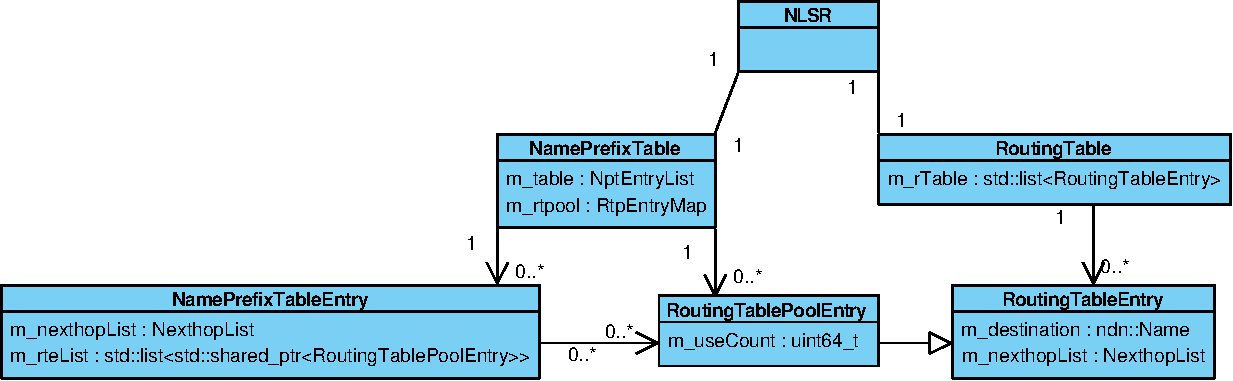
\includegraphics[width=0.8\linewidth]{npt.pdf}
  \begin{caption}
    A diagram of the NPT and Routing Table.

    \begin{footnotesize}
      The ``wire'' arrows represent references (i.e. ``x has y''),
      whereas the ``solid'' arrows represent inheritance (i.e. ``y subclasses x''). \\
      The quantification (e.g. 0..*) is standard UML.
    \end{footnotesize}
  \end{caption}
  \label{fig:npt-class-diagram}
\end{figure}

The Name Prefix Table (NPT) is used by NLSR to maintain a list of all known name prefixes advertised by other routers, including router names.
The NPT maintains a collection of NPT entries, where each entry represents a name prefix and all of its associated routing table entries.
Additionally, to optimize the storage and association of the routing table entries, the NPT also maintains a collection of duplicated routing table entries, called routing table pool entries, which have an additional use count attribute.
The NPT entries keep shared pointers to the appropriate routing table pool entries.
If a name prefix is advertised by multiple routers, the name prefix will be represented by only one Name Prefix Table Entry, but will have multiple routing table pool entries  which correspond with each origin router.

If a Name LSA exists with some advertised name prefix, then that prefix must have an entry in the NPT. So, if two routers advertise the same name prefix, i.e. their name LSAs contain a common name prefix, even if one router withdraws that common name prefix, the entry must remain in the NPT, because the other router still advertises it.

If any type of LSA for a remote router exists in the LSDB, the remote router's name prefix must be in the NPT.
An NPT Entry for a router name can only be removed when there are no more LSAs in the LSDB from the origin router. Note, even if some NPT entry nas no next hops, it will \emph{not} be removed from the NPT; it may later become possible to route to this prefix. These prefixes will be removed from the FIB, however.

\subsection{Adding an NPT Entry}
\label{sec:npt-add}
The \texttt{NamePrefixTable::addEntry()} method is the public
interface for name prefixes to be added to the NPT.
The name prefix as well as the router's prefix which originates the
name prefix are passed as parameters to the method.

If the name prefix is new, there will be no NPT entry for it, so one
will be created. If the name prefix is not new, the existing entry
will be updated, so the existing entry will also store this new origin
router's prefix, too. If after updating, the NPT entry has any next
hops, which are associated to each of the origin router prefixes, the
NPT will update the FIB to include that prefix and its next hops. The
next hop list is sorted and truncated to be only as long as the
\texttt{max-faces-per-prefix} variable.
n
\subsection{Removing an NPT Entry}
\label{sec:npt-del}
The \texttt{NamePrefixTable::removeEntry()} method is the public
interface for name prefixes to be removed from the NPT.
The name prefix as well as the router's prefix which originates the
name prefix are passed as parameters to the interface.

This method removes an origin router prefix from some advertised name
prefix. After this, there may be other origin routers that serve this
name prefix, so this does not guarantee that the NPT entry will be
deleted. If after updating the entry has any next hops, the NPT will
update the FIB to reflect the change. Since the next hop list is
sorted by ascending cost and its length truncated to
\texttt{max-faces-per-prefix}, the contents of next hop list will not
change if the removed origin router prefix was not already in the list
passed to the FIB.

Note that even if the entry no longer has any next hops, it will be retained. All FIB entries for this prefix will be removed from the FIB, which will result in unregistrations from NFD, but the NPT entry will be retained. This is because it may become possible later to route to these origin routers again.

\subsection{Updating an NPT Entry with New Routing Table Entries}
\label{sec:npt-update-with-new-route}
When the Routing Table module has finished calculating, it will notify
the NPT using the \texttt{NamePrefixTable::updateWithNewRoute()}
method.
The NPT will then make approximately $m \times n$ calls to
\texttt{addEntry}, where $m$ is the number of NPT entries and $n$ is
the number of origin routers for each m. That is, $n$ will vary from
one NPT entry to the next in most cases.

\subsection{Routing Table Entry Pool}
The Name Prefix Table has an internal data structure to help
de-duplicate Routing Table information. Without this, each Routing
Table entry has to be stored $n$ times, if $n$ is the number of
prefixes that origin router advertises. Instead, each time a Routing
Table entry would be fetched, the NPT first checks its internal data
structure to see if that Routing Table entry is being used by another
NPT entry. In that case those two NPT entries can share a pointer to
that cached copy of the Routing Table entry.

This internal cache is smart, and will clean up from the cache unused
entries when they are removed from the last NPT entry.

\clearpage
\section{FIB Interaction}
\label{sec:fib}

The FIB module interacts directly with NFD to perform registrations and unregistrations of name prefixes.
The FIB module is notified of additions, removals, or updates to the Name Prefix Table and will use the updated Name Prefix Table to perform the necessary registrations or unregistrations.
The Name Prefix Table notifies the FIB module using the \texttt{Fib::update()} method which accepts a name prefix and next hops for that name prefix as parameters.
The FIB module maintains a shadow FIB which represents its expectations of NFD's FIB.
The FIB module uses the shadow FIB to determine which registrations and unregistrations are necessary.

\subsection{Updating the FIB}
When the Name Prefix Table performs an update on the FIB module, the FIB module will first sort the passed next hops with the next hop's costs in increasing order.
The FIB module will next determine the number of next hops that should be installed for the name prefix using the \texttt{max-faces-per-prefix} parameter as a maximum.
If there are more passed next hops than the \texttt{max-faces-per-prefix} parameter allows, the FIB module will only use the first \texttt{max-faces-per-prefix} number of next hops from the sorted list.
If there are less passed next hops than the \texttt{max-faces-per-prefix} parameter, the FIB module will use all of the passed next hops.

The FIB module next determines if there is already a FIB entry in the shadow FIB for the passed name prefix.
If the name prefix will create a new FIB entry and the number of passed next hops is greater than zero, a new FIB entry will be created,
the next hops will be registered for the name prefix in NFD's FIB, and the FIB entry will be set to expire in two times the \texttt{lsa-refresh-time} in order to clean up orphaned entries in NFD's FIB.
If there is already an existing FIB entry for the name prefix and the number of passed next hops is greater than zero, any of the passed next hops that weren't previously registered for the FIB entry are registered.
Then, any currently registered hops that are not in the passed next hops are removed from NFD's FIB, and the entry's expiration is refreshed.
If there is already an existing FIB entry for the name prefix and the number of passed next hops is equal to zero, the routing table was unable to find a path to this name prefix and so the name prefix should be removed from NFD's FIB.

\clearpage
%\section{Sequencing Manager}
\label{sec:sequencing-manager}

%\section{Prefix Update Processor}
\label{sec:prefix-update}

%\section{Dataset Publishers}
\label{sec:publishers}

\section{Security}
\label{sec:security}

The trust model of NLSR is semi-hierarchical. An example certificate signing hierarchy is show in Figure~\ref{fig:trust}.
In this hierarchy, each entity's name and corresponding certificate name follow the convention described in Table~\ref{table:kname}.

\begin{figure}
\centering
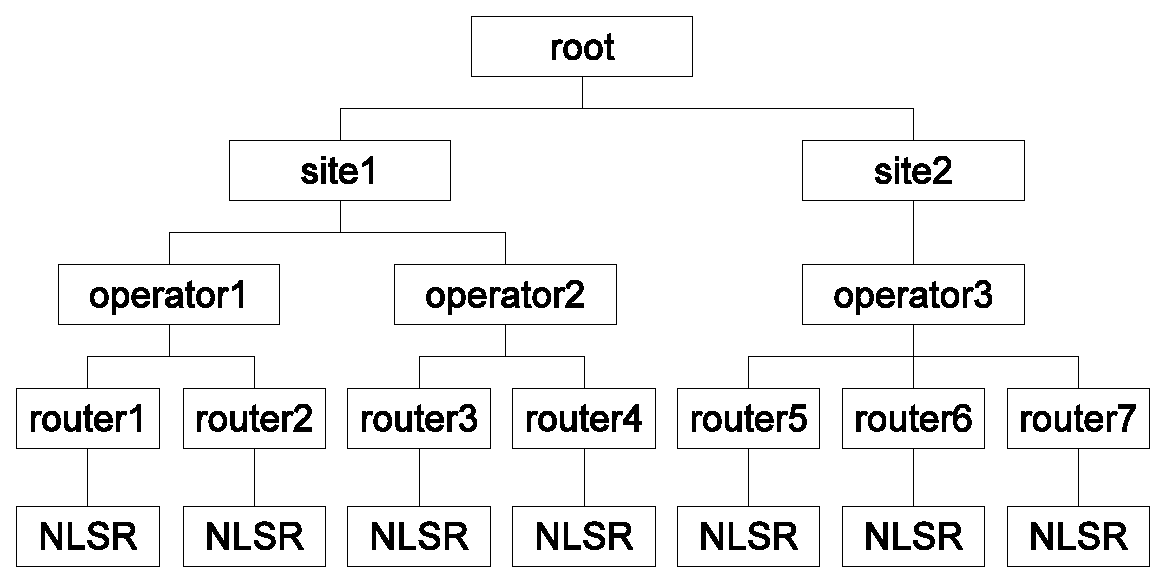
\includegraphics[width=0.5\linewidth]{figures/trust-hierarchy.eps}
\caption{NLSR Trust Hierarchy}
\label{fig:trust}
%\vspace{-3mm}
\end{figure}

\begin{table}
\centering	
	\caption{Key Names}
	\small
	\begin{tabular}{|l|l|}
	\hline
	\bfseries {Key Owner} & \bfseries {Key Name}\\ \hline
	Network & /$<$network$>$/KEY/$<$key$>$\\ \hline
	Site & /$<$network$>$/$<$site$>$/KEY/$<$key$>$\\ \hline
	Operator & /$<$network$>$/$<$site$>$/$<$operator$>$/KEY/$<$key$>$\\\hline
	Router & /$<$network$>$/$<$site$>$/$<$router$>$/KEY/$<$key$>$\\\hline
	NLSR & /$<$network$>$/$<$site$>$/$<$router$>$/NLSR/KEY/$<$key$>$\\\hline
	\end{tabular}
	\label{table:kname}
	\vspace{-3mm}
\end{table}

\subsection{Creating Keys and Certificates}

The process to create keys and certificates for this hierarchy can be performed using the \texttt{ndnsec}~\cite{ndnsec} tools included with \texttt{ndn-cxx}~\cite{NDNCXX}.
The steps to create the keys and certificates is outlined below:

\begin{enumerate}
\item Create keys for Root: \\ \texttt{ndnsec-keygen \$ROOT\_NAME > \$ROOT\_KEY\_OUTPUT\_FILE}
\item Create certificate for Root: \\ \texttt{ndnsec-certgen -N \$ROOT\_NAME -p \$ROOT\_NAME \$ROOT\_KEY\_OUTPUT\_FILE > \$ROOT\_CERT\_OUTPUT\_FILE}
\item For each site, create keys and certificates:
  \begin{enumerate}
  \item On the Site machine, generate keys for the Site: \\ \texttt{ndnsec-keygen \$SITE\_NAME > \$SITE\_KEY\_OUTPUT\_FILE}
  \item Copy \texttt{\$SITE\_KEY\_OUTPUT\_FILE} over to the machine where the Root certificate was created.
  \item Generate a certificate for the Site on the Root machine: \\ \texttt{ndnsec-certgen -N \$SITE\_NAME -p \$SITE\_NAME -s \$ROOT\_NAME \$SITE\_KEY\_OUTPUT\_FILE > \$SITE\_CERT\_OUTPUT\_FILE}
  \item Copy \texttt{\$SITE\_CERT\_OUTPUT\_FILE} over to the Site machine.
  \item Install the certificate on the Site machine: \\ \texttt{ndnsec-cert-install -f \$SITE\_CERT\_OUTPUT\_FILE}
  \item On the Site machine, create the Operator keys: \\ \texttt{ndnsec-keygen \$OP\_NAME > \$OP\_KEY\_OUTPUT\_FILE}
  \item On the Site machine, create the Operator certificate: \\ \texttt{ndnsec-certgen -N \$OP\_NAME -p \$OP\_NAME -s \$SITE\_NAME \$OP\_KEY\_OUTPUT\_FILE > \$OP\_CERT\_OUTPUT\_FILE}
  \item On the Site machine, create the Router keys: \\ \texttt{ndnsec-keygen \$ROUTER\_NAME > \$ROUTER\_KEY\_OUTPUT\_FILE}
  \item On the Site machine, create the Router certificate: \\ \begin{small}\texttt{ndnsec-certgen -N \$ROUTER\_NAME -p \$ROUTER\_NAME -s \$OP\_NAME \$ROUTER\_KEY\_OUTPUT\_FILE > \$ROUTER\_CERT\_OUTPUT\_FILE}\end{small}
  \end{enumerate}
  \item When NLSR starts, it will automatically create the NLSR keys and certificates for the router.
\end{enumerate}

\subsection{Certificate Publishing}

In a network, every router must have the root certificate configured as a trust anchor for the \texttt{validator} in the configuration file. If two routers in a network do not share a common trust anchor, then when one seeks to validate the data of the other, they may be unable to establish trust in their signature. This is, of course, because of how the trust hierarchy is set up: you trust the person that signed some router's certificate, because it was signed by the site certificate, and the site certificate was signed by the region, etc., and the $nth$ certificate was signed by the root certificate, which is your trust anchor, so you ``just trust it''. Moreover, if your trust anchor is \emph{before} their trust anchor in the ``chain'', then they will be able to trust you, but you will not be able to trust them.

For each site, at least one router should publish the site certificate, and at least one router should publish the certificate of the site operator.
Each router should publish its own certificate. This is a matter of performance; a network would work if all certificates for all nodes were kept centrally, but distributing the certificates in this way improves performance.
All this information must be explicitly specified in the configuration file.

For example, the following configuration file indicates that NLSR should publish the site certificate and the router certificate:

\begin{verbatim}
...
security
{
  validator
  {
    ...
  }
  cert-to-publish "$SITE_CERT_OUTPUT_FILE"   ; name of the site certificate file
  cert-to-publish "$SITE_CERT_OUTPUT_FILE"   ; name of the router certificate file
  ...
}
\end{verbatim}

\clearpage
\section{Configuration File}
\label{sec:configuration}

NLSR's configuration file contains numerous parameters to control the behavior and performance of NLSR.
The configuration file also includes the trust schema used by NLSR to verify LSA Data, Hello Data, and prefix update command Interests.
The configuration file is divided into six sections each with parameters that mainly affect a specific module.

\subsection{General Section}

The \texttt{general} section in the configuration file includes parameters which deal with the general setup of the router, the behavior of the LSDB, and logging configuration.

There are three parameters used to configure the router prefix of the router.
The router prefix is the name that other routers in the network know this router by.
\begin{itemize}
\item \texttt{network} - the name of the network to which the router belongs; e.g., \texttt{/ndn}.
\item \texttt{site} - the name of the site to which the router belongs; e.g., \texttt{/edu/memphis}.
\item \texttt{router} - the name to identify the router; e.g., \texttt{/\%C1.Router/cs/pollux}.
\end{itemize}
The router prefix is constructed by combining the three parameters following the format: \texttt{/<network>/<site>/<router>}.

There are three parameters which affect the behavior of the LSDB.
\begin{itemize}
\item \texttt{lsa-refresh-time} - the time in seconds the router will wait before refreshing its LSAs (Default value: 1800; Valid values: 240 - 7200).
\item \texttt{router-dead-interval} - the time in seconds after which an inactive router's LSAs are removed.
The configured value for this parameter must be greater than \texttt{lsa-refresh-time}. (Default value: two times the value configured in \texttt{lsa-refresh-time}).
\item \texttt{lsa-interest-lifetime} - the interest lifetime used for LSA Interests (Default value: 4; Valid values: 1 - 60).
\end{itemize}

The \texttt{log-level} parameter configures the verbosity of NLSR's logging.
The possible \texttt{log-level} values are listed in increasing verbosity:
\begin{itemize}
\item \texttt{NONE} - no messages
\item \texttt{ERROR} - error messages
\item \texttt{WARN} - warning messages
\item \texttt{INFO} - informational messages (default)
\item \texttt{DEBUG} - debugging messages
\item \texttt{TRACE} - trace messages (most verbose)
\item \texttt{ALL} - all messages
\end{itemize}
Note that all debugging levels listed above the selected value will also be enabled.

The \texttt{general} configuration section also includes parameters to choose where the NLSR log file and the NLSR sequence number file are stored.
The \texttt{log-dir} parameter is an absolute path to the directory where the NLSR log file should be written, and \texttt{seq-dir} is an absolute path to the directory where the NLSR sequence number should be written.

\subsection{Neighbors Section}

The \texttt{neighbors} section in the configuration file contains parameters that define the behavior of the Hello Protocol and the neighboring routers of the router.
\begin{itemize}
\item \texttt{hello-retries} - the number of times to retry a Hello Interest before deciding the neighbor is down (Default value: 3; Valid values: 1 - 10).
\item \texttt{hello-timeout} - the interest lifetime for Hello Interests in seconds (Default value: 1, Valid values: 1 - 15).
\item \texttt{hello-interval} - the time in seconds between sending each Hello Interest to a neighbor. (Default value: 60; Valid values: 30 - 90).
\item \texttt{first-hello-interval} -  the time to wait in seconds before sending the first Hello Interests (Default value: 10; Valid values: 0 - 10).
\item \texttt{adj-lsa-build-interval} - when the Hello Protocol triggers an Adjacency LSA build, the LSDB will wait this amount of time in seconds before performing the Adjacency LSA build. This parameter is intended to allow for Adjacency LSA build requests to be aggregated and the build can then be performed once. (Default value: 5; Valid values: 0 - 5)
\end{itemize}

The \texttt{neighbors} section also includes multiple \texttt{neighbor} subsections, each of which configures a neighbor of the router.
The \texttt{neighbor} subsection includes:
\begin{itemize}
\item \texttt{name} - the router prefix of the neighboring router
\item \texttt{face-uri} - the face that should be used to connect to the neighboring router
\item \texttt{link-cost} - the cost metric for the link connecting this router to the neighbor router.
\end{itemize}

\subsection{Hyperbolic Section}

The \texttt{hyperbolic} section in the configuration file is used to enable/disable hyperbolic routing and to specify the hyperbolic coordinates of the router.

The \texttt{state} parameter indicates whether or not hyperbolic routing should be enabled. There are three possible values for this parameter: \texttt{on}, \texttt{off}, and \texttt{dry-run}. \texttt{on} enables hyperbolic routing; \texttt{off} disables hyperbolic routing (link-state routing is used); \texttt{dry-run} uses link-state routing to populate NFD's FIB, but will also perform the hyperbolic routing calculations and write them to the log file for debugging purposes.

The \texttt{radius} parameter defines the router's radius in the hyperbolic coordinate system and \texttt{angle} defines the router's angle in the hyperbolic coordinate system.

\subsection{FIB Section}

The \texttt{fib} section in the configuration file contains two parameters: one to limit the number of next hops registered for each name prefix, and the amount of time to wait before calculating the routing table after a request is made.

\texttt{max-faces-per-prefix} defines the maximum number of next hops that can be registered for a name prefix.
This value is intended to reduce the FIB size for routers with a large number of neighbors.
The default value for \texttt{max-faces-per-prefix} is \texttt{0} which indicates that all available next hops may be added to each name prefix. \texttt{max-faces-per-prefix} allows values between 0 and 60.

\texttt{routing-calc-interval} is the time to wait in seconds after a routing table calculation is requested before actually performing the routing table calculation.
This parameter is intended to limit the number of routing table calculations, which may be performance intensive on some systems.
The default value for \texttt{max-faces-per-prefix} is 15 seconds and can be configured to be in the range of 0 to 15 seconds.

\subsection{Advertising Section}

The \texttt{advertising} section includes a list of name prefixes that the router should advertise as reachable through itself.
Each name prefix that should be advertised should be in the following format: \texttt{prefix /name/to/advertise}.
This section allows for static configuration of the advertised prefixes, but prefixes can be dynamically advertised and withdrawn using the Prefix Update Processor. 

\subsection{Security Section}

The \texttt{security} section of the configuration file includes the configuration for NLSR's validators and the locations of certificates that should be published by the router.

The \texttt{validator} subsection includes the configuration for the validator used by NLSR to verify the signatures of Hello Data and LSA Data.

The \texttt{prefix-update-validator} configures the validator used by the Prefix Update Processor to verify that prefix update command Interests are signed by the operator of the router.

The \texttt{security} section also allows configuration of which certificates should be published by the router using the \texttt{cert-to-publish} keyword.
If the router should publish a certificate, the absolute path for the certificate file can be configured as \texttt{cert-to-publish} value.

\clearpage

\phantomsection
\addcontentsline{toc}{section}{References}

\bibliographystyle{IEEEtran}
\bibliography{nlsr}

\end{document}
